\documentclass{beamer}
\usetheme{Madrid}

\usepackage{amsmath, amssymb, amsthm}
\usepackage{graphicx}
\usepackage{gensymb}
\usepackage[utf8]{inputenc}
\usepackage{hyperref}
\usepackage{tikz}


\title{4.12.17 Matgeo}
\author{AI25BTECH11012 - Garige Unnathi}
\date{}

\begin{document}

\frame{\titlepage}

% Question frame
\begin{frame}
\frametitle{Question}
\textbf{$P_1$},\textbf{$P_2$} are points on either of the two lines y - $\sqrt{3}$$\lvert x \rvert$ $=$ 2 at a distance of 5 units from their point of intersection. Find the coordinates of the foot of the perpendiculars drawn from \textbf{$P_1$},\textbf{$P_2$} on the bisector of the angle between the given lines.\\
\end{frame}


% Solution steps
\begin{frame}
\frametitle{Solution}
The equation of the lines is :
\begin{align}
  y - \sqrt{3}x = \begin{bmatrix}-\sqrt{3} & 1\end{bmatrix}\begin{bmatrix}x\\y\end{bmatrix} = 2\\
   y + \sqrt{3}x = \begin{bmatrix}\sqrt{3} & 1\end{bmatrix}\begin{bmatrix}x\\y\end{bmatrix} = 2 
\end{align}
Combining both the equations 0.1 and 0.2 ,we get :
\begin{align}
   \begin{bmatrix}-\sqrt{3} & 1\\
           \sqrt{3} & 1 \end{bmatrix}\textbf{X} = \begin{bmatrix}2\\2\end{bmatrix}
\end{align}
Solving by row reduction we get :
\begin{align}
\textbf{Q} = \begin{bmatrix}0\\2\end{bmatrix}
\end{align}
\end{frame}



\begin{frame}
\frametitle{Solution}
The equation for the point $\mathbf{P_1}$ are:
\begin{align}
\begin{bmatrix}-\sqrt{3} & 1\end{bmatrix}\mathbf{P_1} = 2\\
\lVert P_1 - Q \rVert = 5
\end{align}

The equation for the point $\mathbf{P_2}$ are:

\begin{align}
\begin{bmatrix}\sqrt{3} & 1\end{bmatrix}\mathbf{P_2} = 2\\
\lVert P_2 - Q \rVert = 5
\end{align}

Solving the equations we get :
\begin{align}
   \mathbf{P_1} = \begin{bmatrix}\frac{5}{2} \\ 2+\frac{5\sqrt{3}}{2}\end{bmatrix} \\
    \mathbf{P_2} = \begin{bmatrix}-\frac{5}{2} \\ 2-\frac{5\sqrt{3}}{2}\end{bmatrix}
\end{align}
\end{frame}

\begin{frame}
\frametitle{Solution}
The equation of the angle bisector is given by \\
Let us take a point \textbf{P} on the angle bisector , substitution it in the line equtions and equating the angles we get the equation :
\begin{align}
  \frac{\lvert n_1\textbf{P} - 2 \rvert}{\lVert n_1\rVert}  =  \frac{\lvert n_2\textbf{P} - 2 \rvert}{\lVert n_1\rVert} \\
  \frac{n_1\textbf{P} - 2}{\lVert n_1\rVert} \pm \frac{ n_2\textbf{P} - 2}{\lVert n_1\rVert} = 0
\end{align}
solving the above equation we get locus of $\vec{P}$ as two lines which are the angle bisectors :

\begin{align}
    \begin{bmatrix}1\\0\end{bmatrix}^{T}\textbf{x} = 0\\
     \begin{bmatrix}0\\1\end{bmatrix}^{T}\textbf{x} = 2
\end{align}

\end{frame}
\begin{frame}
\frametitle{Solution}
Let Q be the foot of the perpendicular from P to the line
\begin{align}
    \textbf{n}^{T}\textbf{x} = c
\end{align}
Then :
\begin{align}
    \begin{bmatrix}\textbf{m}&\textbf{n}\end{bmatrix}^{T}\textbf{Q} = \begin{bmatrix}\textbf{m}^{T}\textbf{P}\\c\end{bmatrix}
\end{align}

solving this equation for the line $\begin{bmatrix}1\\0\end{bmatrix}^{T}\textbf{x} = 0$ ,we get :
\begin{align}
    \begin{bmatrix}0\\2+\frac{5\sqrt{3}}{2}\end{bmatrix} \quad and \quad \begin{bmatrix}0\\2-\frac{5\sqrt{3}}{2}\end{bmatrix}
\end{align}
and solving it for the line $\begin{bmatrix}0\\1\end{bmatrix}^{T}\textbf{x} = 2$, we get :
\begin{align}
    \begin{bmatrix}\frac{5}{2} \\ 2\end{bmatrix} \quad and \quad \begin{bmatrix}-\frac{5}{2} \\ 2\end{bmatrix}
\end{align}


\end{frame}
% Graphical representation
\begin{frame}

\frametitle{Graphical Representation}
\begin{center}
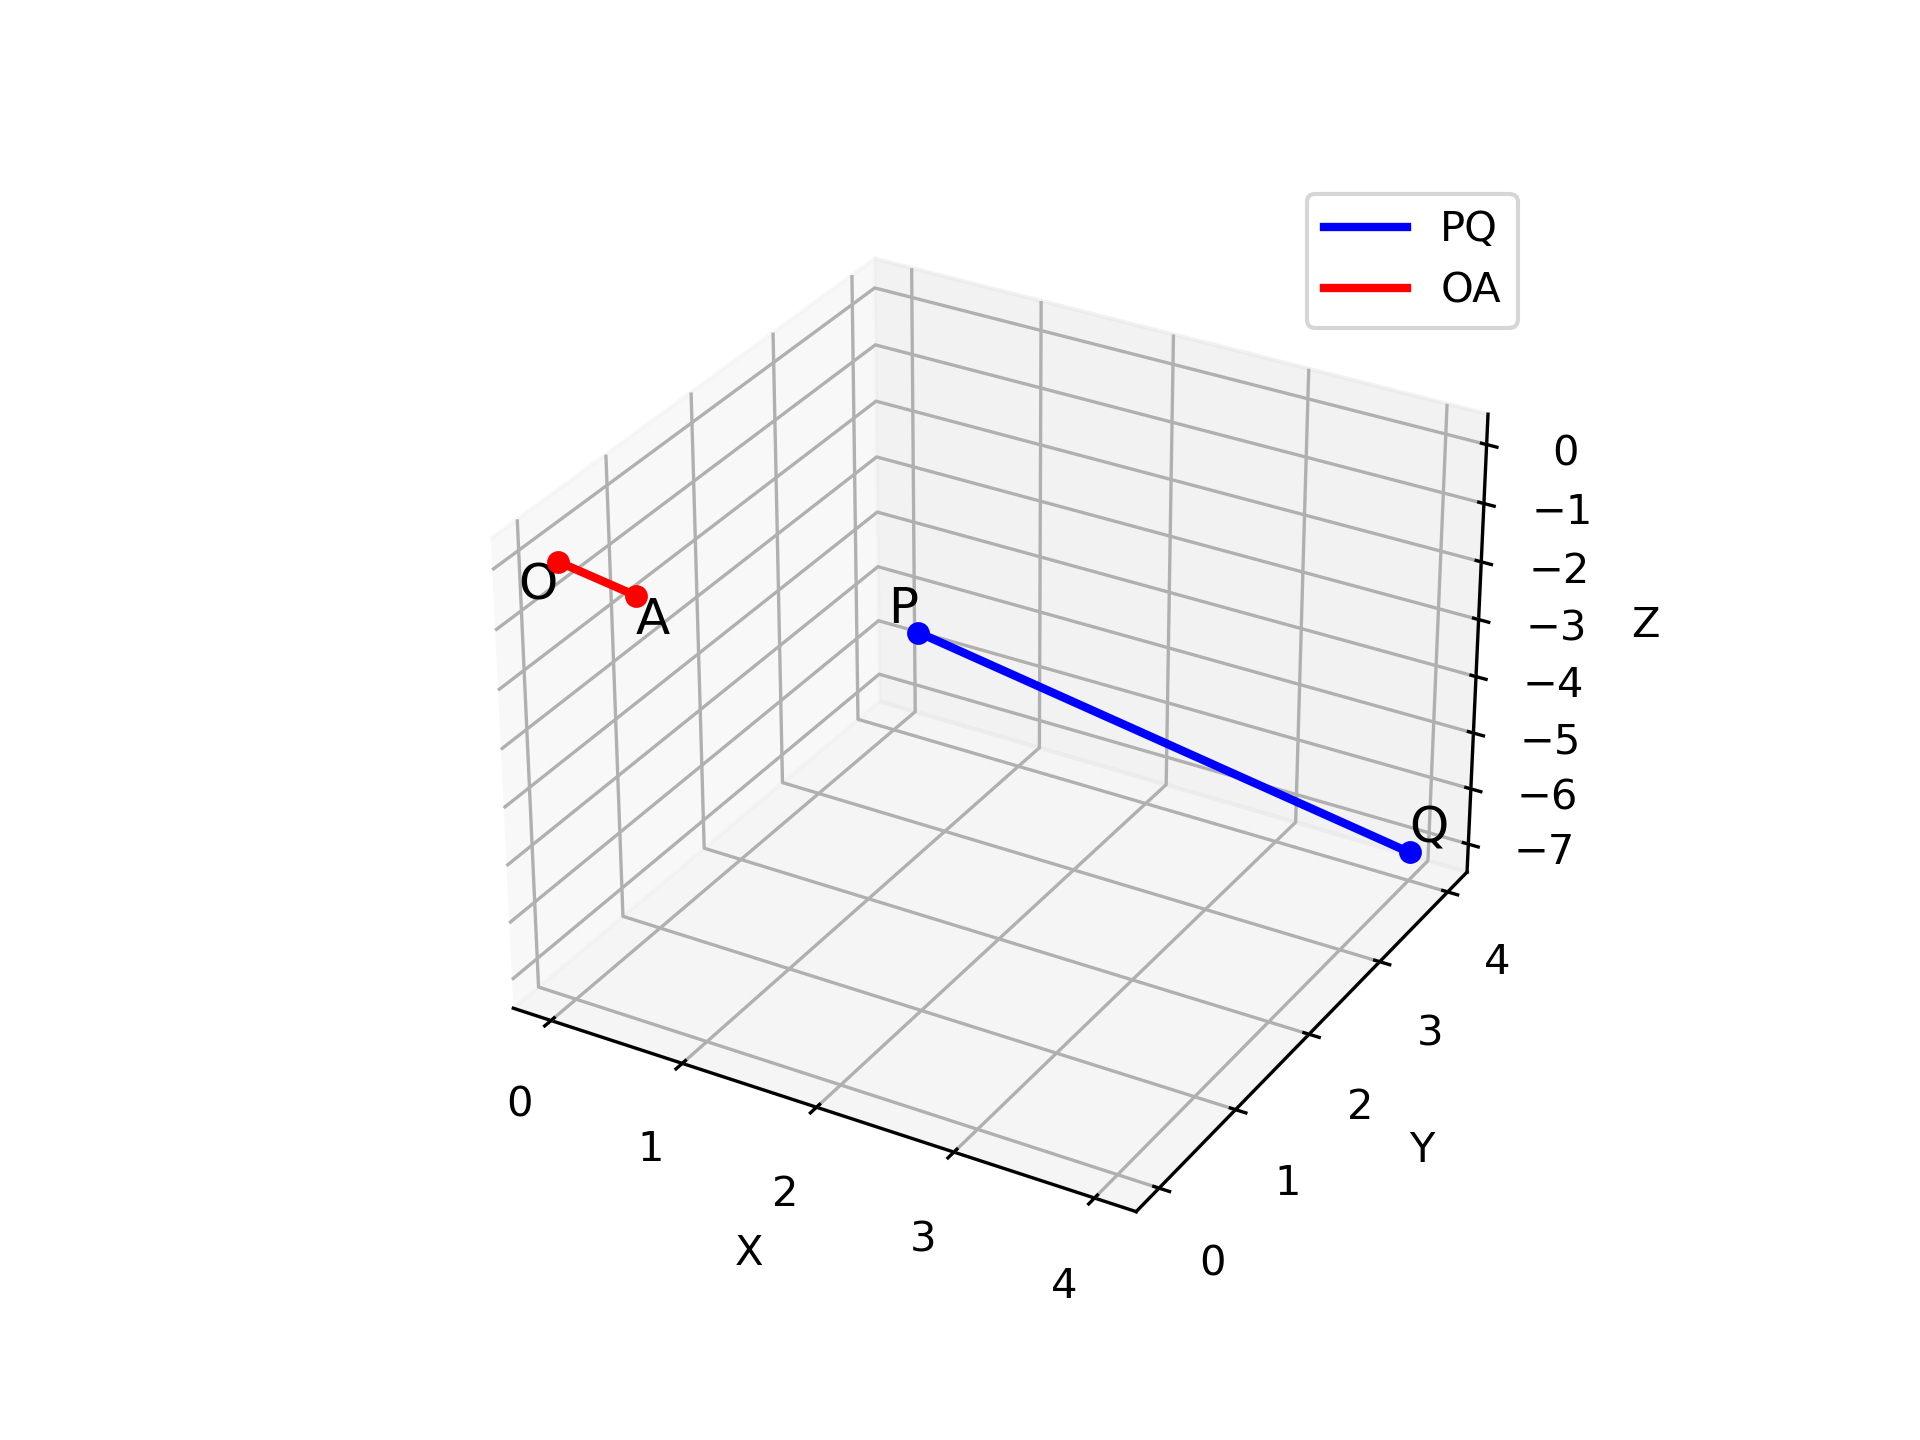
\includegraphics[width=0.6\linewidth]{/Users/unnathi/Documents/ee1030-2025/ai25btech11012/matgeo/4.12.17/figs/fig.png}
\end{center}
\end{frame}

\end{document}
